% 8. előadás második fele, 9. előadás első fele

\chapter{Az Intel Netburst architektúra}

\section{Bevezetés}
A második generációs szuperskalárok fejlesztése során a 90-es évek második felében elérték az architektúra teljesítménybeli korlátait.
A hatékonyság növelésének extenzív forrásai kimerültek.
A sebesség további fokozásához a következő módszerekkel keresték a megoldást:
\begin{itemize}
    \item új architektúrák, pl. VLIW (ld. \ref{vliw}. fejezet)
    \item párhuzamosság egyéb forrásai (szál vagy folyamat szintű párhuzamosság)
    \item frekvencia erőteljes növelése
\end{itemize}
Az Intelnél a frekvencia erőteljes növelésével próbálkoztak, de az akkori legfejlettebb architektúrájuk, a P6 (Pentium III alapja) nem volt alkalmas 1333 MHz fölötti működésre.
A fejlesztés során a 10 GHz elérését tűzték ki célul, így új architektúra kellett.
Ez lett a Netburst architektúra, amire a Pentium IV processzorcsalád épült.
Az architektúra nem jelentette a második, illetve harmadik generációs szuperskalárok gyökeres újratervezését, a célkitűzés mindössze a magasabb frekvenciás működés volt.

\section{A frekvencia növelése}
A frekvencia növeléséhez a következő változtatásokat vezették be:
\begin{itemize}
    \item Gyártási csíkszélesség csökkentése (180 nm $\rightarrow$ 65 nm), általában egy lépésben 0.7-szeresére csökkentik (így fele akkora helyen fér el ugyanannyi tranzisztor, mint a korábbi technológiánál, tehát a tranzisztorok száma megduplázható $\rightarrow$ Moore-törvény).
    \item Futószalag fokozatok hosszának csökkentése (ennek egyik módja a fokozatok kisebb részekre bontása, viszont ekkor a fokozatok száma növekszik, nő a párhuzamosan végrehajtott utasítások száma és a függőségek száma is $\rightarrow$ csökkenhet a hatékonyság).
\end{itemize}

\section{Jellemzői}
\begin{itemize}
    \item CISC architektúra (1-17 byte hosszú utasítások)
    \item belső RISC mag
    \item hosszabb futószalagok (több függőség, de magasabb frekvencia)
\end{itemize}

\section{Újdonságok}

\subsection{Execution Trace Cache}
Az Execution Trace Cache az L1 utasítás cache-nek felel meg, de CISC helyett már dekódolt RISC utasításokat tartalmaz a végrehajtásuk feltételezett sorrendjében.

\subsection{Hyper futószalag}
A Hyper futószalag lényege, hogy a dekódoló fokozat nincs benne.
A dekódolás futószalagon kívül történik, azért, hogy az L1 cache-ben (Execution Trace Cache) már dekódolt és átalakított utasítások szerepelhessenek.
Oka, hogy a CISC utasítások átalakítása lassú, akadályozta volna a nagy frekvenciás végrehajtást, ezért külön került a futószalagtól.
Újdonság még, hogy a korábbi 10-15 fokozathoz képest 20-31 fokozatot tartalmazott.
Ennek hátránya, hogy hibás becslés esetén nagyobb a büntetés, több fokozatot kell törölni a futószalagból $\rightarrow$ fajlagos teljesítmény csökkenés.

\subsection{Enhanced Branch Prediction}
Ez egy továbbfejlesztett elágazásbecslő logika, 94-97 \%-os hatékonysággal (PIII-hoz képest kb. 33 \%-al csökkent a hibás becslések száma).

\subsection{Quad Data Rate Bus}
A Quad Data Rate Bus egy belső rendszerbusz, gyorsítja az adatelérést az L1 és L2 gyorsítótárak felé.
A buszfrekvencia négyszeresén továbbítja az adatokat (a külső rendszerbusz sebességét nem lehetett növelni, mivel a memória nem gyosult jelentősen). Ennek eléréséhez kettő órajel generátort alkalmaz, 90\textdegree-os fáziseltolással, valamint a felfutó és lefutó élen is történik adattovábbítás.
Így óraciklusonként négy adattovábbítás történik.
Ezt a működést mutatja be a \ref{fig:qdrb}. ábra.
\begin{figure}[h]
    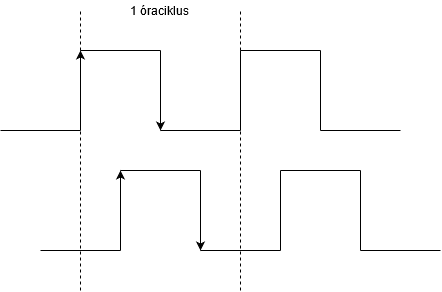
\includegraphics[width=0.6\textwidth]{qdrb}
    \centering
    \caption{A Quad Data Rate Bus kettős órajele}
    \label{fig:qdrb}
\end{figure}

\subsection{Rapid Execution Engine}
A Rapid Execution Engine az egyszerű FX műveletek gyors végrehajtására szolgáló végrehajtó egység.
Az órajel felfutó és lefutó élére is képes műveletvégzésre, így a végrehajtási idő akár egy fél ciklusra is csökkenhet.
A gyorsaság érdekében kevesebb kaput tartalmaz, csak az alapműveletek elvégzésére képes.
Ez sikeres lett, nőtt a hatékonyság, később kettőt is beépítettek a CPU-kba.

\subsection{Replay System}
Probléma, hogy a sok fokozatú futószalag sok függőséggel jár, ami az utasítások várakozását és kihasználatlanságot eredményezhet.
Ennek megoldására az ütemező megbecsüli az utasítások végrehajtási idejét, így tudja, hogy az utasítás végrehajtásának kezdetétől mennyi idő múlva fogja igényelni a bemenő operandust.
Ezért a függő utasítást már ennyi idővel a szükséges függőség teljesülése előtt kiküldi, hogy pont mire felhasználná a bemenő operandust, az már éppen előállt.
Ha rossz volt a becslés és hamarabb szükség lenne a forrás operandusra, mint ahogy az előállt, az utasítás egy speciális sorba, a Replay Queue-ba kerül, ahonnan később újra kiküldésre kerül.
Bár a hatékonyságot mindez csökkenti, elkerülhető a futószalag leállása, így biztosítja a végrehajtó egységek optimális kihasználását.

\section{Következmény}
A fajlagos teljesítmény, azaz az IPC (Instructions Per Cycle) csökken. Ez összességében nem jelenti viszont a teljesítmény csökkenését, mivel az órajel magasabb lett (több ciklus időegység alatt).

\section{Fejlődési korlátok}

\subsection{Statikus disszipáció}
Problémát jelentett a szivárgási áram exponenciális növekedése a frekvencia emelésével (statikus disszipáció).
A szivárgási áram létrejön, mivel a tranzisztorokon akkor is folyik valamennyi áram, amikor az kikapcsolt állapotban van.
A szivárgási áram fajtái:
\begin{itemize}
    \item Gate $\rightarrow$ Drain
    \item Source $\rightarrow$ Drain
\end{itemize}
A statikus disszipáció miatt növekedett a hőtermelés, 3.8 - 4 GHz környékén bekövetkezett a hőkatasztrófa (1 cm\textsuperscript{2}-en 100 W disszipáció). Ennek kezelése hagyományos eszközökkel nem megvalósítható, csak vízhűtéssel, ami viszont nem gazdaságos.
A statikus disszipáció kiszámítása:
\begin{center}
    $D\textsubscript{s}=V*I\textsubscript{leak}$,
\end{center}
ahol $V$ a feszültség, $I\textsubscript{leak}$ pedig a szivárgási áram, ami a frekvencia növekedésével exponenciálisan nő.

\subsection{Dinamikus disszipáció}
Az a disszipáció, amit az aktív tranzisztorokon átfolyó áram hőtermelése okoz.
A dinamikus disszipáció kiszámítása:
\begin{center}
    $D\textsubscript{d}=A*C*V^2*f\textsubscript{c}$,
\end{center}
ahol $A$ az aktív kapuk száma, $c$ a kapuk összesített elosztott kapacitása, $v$ a tápfeszültég, $f\textsubscript{c}$ pedig a magfrekvencia.
Látszik, hogy a dinamikus disszipáció négyzetesen függ a feszültségtől, így a frekvencia növelése a feszültség csökkentésével ellensúlyozható.

\subsection{Teljes disszipáció}
A teljes disszipáció a statikus és a dinamikus összege.
A frekvencia növelésével egyre jelentősebbé vált a dinamikus disszipáció, arányaik változása:
\begin{center}
    \begin{tabular}{c | c | c}
             & D\textsubscript{s} & D\textsubscript{d} \\
        \hline
        1995 & 1                  & 10000              \\
        \hline
        2005 & 1                  & 1                  \\
    \end{tabular}
\end{center}
Ezért jelentek meg az új tranzisztor technológiák.

\subsection{Párhuzamos buszok frekvencia korlátja}
A buszokon logikai 1-esek és 0-k közlekednek. Annak, hogy az érzékelők ezeket a jeleket meg tudják különböztetni, időbeli és feszültségbeli fetételei vannak.
Ezt írja le a Data Valid Window fogalma: ahhoz, hogy az érzékelő egy jelet érvényesnek tekintsen, a jelnek egy bizonyos feszültség intervallumba kell esnie és egy bizonyos ideig fenn kell állnia.
A DVW a \ref{fig:dvw}. ábrán látható, itt a pirossal ábrázolt területbe nem szabad beleesnie a jelnek, hogy érvényes legyen.
Ez gátolja a feszültség csökkentésének lehetőségeit, mivel nagyon kis feszültség esetén a kisebb zavarok is azt eredményezhetik, hogy a jelet ne tekintse érvénytelennek az érzékelő.
A frekvencia is csak bizonyos pontig növelhető, mivel nagy frekvencián a jelek elcsúsznak egymástól, ez a delay skew.
A feszültség növelésével viszont tovább növelhető a frekvencia, mivel a felfutási idő röviebb lesz, meredekebb a felfutási szög, így könnyebb megfelelni az időbeli követelményeknek.
A feszültség (fogyasztás) és a frekvencia (teljesítmény) tehát egymással ellentétes célok, ezért a processzorok gyakran dinamikusan változtatják a feszültség és frekvencia értékeiket: alacsony terhelésen kis feszültség és frekvencia, nagy terhelésen magasabb feszültség és frekvencia.
\begin{figure}[H]
    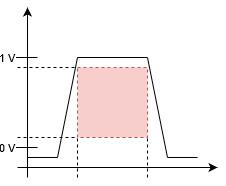
\includegraphics[width=0.4\textwidth]{dvw}
    \centering
    \caption{A Data Validation Window}
    \label{fig:dvw}
\end{figure}

\subsection{Egyéb korlátok}
Megjelentek a párhuzamosság (ILP) hatékonysági korlátai.

\section{A disszipáció csökkentése}
A DVFS (Dynamic Voltage and Frequency Scaling) a dinamikus feszültség és frekvencia szabályozást jelenti (skálázás).
Ez menet közben meghatározza, hogy az adott feladathoz milyen teljesítményre van szükség, majd ehhez igazítja a processzor feszültségét és frekvenciáját.
Példa ilyenre, amikor a mobiltelefon lekapcsolt képernyővel készenléti módban van, majd felvesszük és játszani kezdünk rajta.
Működése:
\begin{enumerate}
    \item szükséges teljesítmény meghatározása
    \item frekvencia hozzáillesztése a szükséges teljesítményhez
    \item órafrekvencia fenntartásához szükséges minimális feszültség beállítása
    \item később kiegészült az AVS-el (Adaptive Voltage Scaling), ez a következő félév anyaga
\end{enumerate}

\section{Az Intel Pentium 4}
A Pentium 4-es CPU 2000-től 2008-ig volt kapható, de a fejlesztését már 2004-ben befejezték, amikor a frekvenciát már nem tudták tovább növelni a statikus disszipáció növekedése miatt.
Kevésbé volt hatékony, mint a korabeli AMD CPU-k, viszont a magasabb órajel miatt nagyobb teljesítményre volt képes.
Míg a Pentium III órajele 500 és 1333 MHz között volt, a P4 1.5 GHz-ről indult és a Prescott architektúrára (2004) elérték a 3.2 GHz-et.

\subsection{Thermal Monitor}
A magasabb frekvenciát a versenytársakéhoz képest jobb hővédelemmel sikerült elérni, ez volt a Thermal Monitor.
Ez egy órajel moduláción alapuló megoldás, ha az érzékelő túlmelegedést észlelt, lekapcsolta (későbbiekben csökkentette) az órajelet.

\subsection{Multimédia}
A P3-hoz képest fejlesztették a multimédiás feldolgozást, 144 új utasítás került be az SSE (FX) és MMX (FP) utasításkészletekbe.

\subsection{Felépítés}
A processzor működési vázlata a \ref{fig:p4}. ábrán látható.
\begin{figure}[h]
    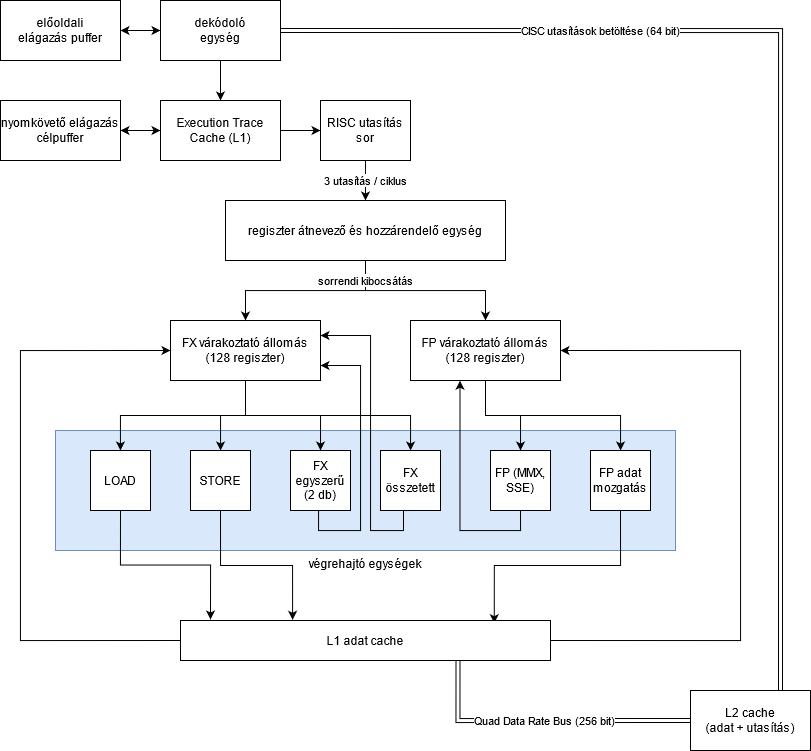
\includegraphics[width=\textwidth]{p4}
    \centering
    \caption{A Pentium 4 processzor működési vázlata}
    \label{fig:p4}
\end{figure}